% Propósito: distinguir los espectros de entrada y salida de la respuesta en
% frecuencia del sistema que los relaciona.
% Origen: Y(f)=X(f)H(f). Se usan magnitudes normalizadas y datos teóricos:
% |X|=(0,8;0,8;0,8), |H|=(1;0,5;0,25) para f=(0,5;1;2) kHz;
% por lo tanto |Y|=(0,8;0,4;0,2).
% Esquema matemático; no representa un dispositivo ni una medición real.
% Descripción accesible: tres paneles muestran, de izquierda a derecha, un
% espectro de entrada con tres componentes iguales, una respuesta de sistema
% que atenúa progresivamente esas frecuencias y un espectro de salida cuyos
% componentes son los productos de entrada y respuesta. La figura enfatiza que
% el espectro pertenece a una señal y H pertenece al sistema.
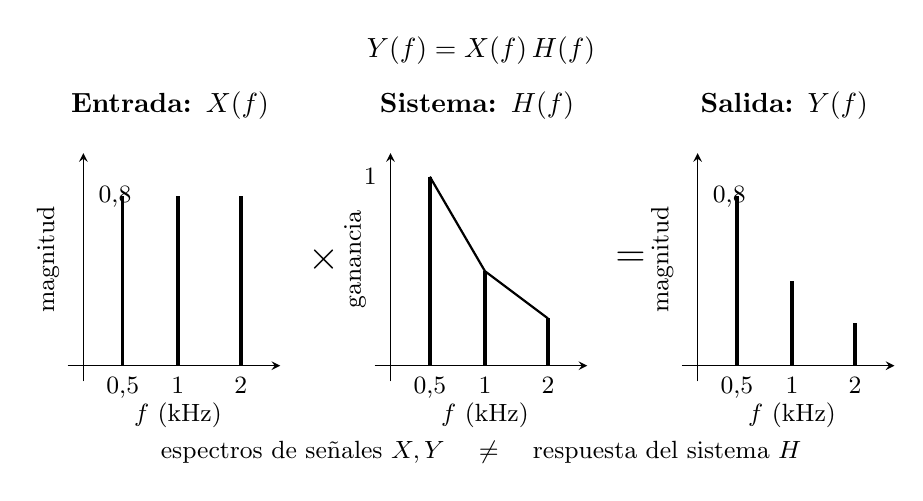
\begin{tikzpicture}[font=\small,>=stealth,x=1cm,y=1cm]
    \node[font=\bfseries] at (5.75,4.75)
        {\(\lvert Y(f)\rvert=\lvert X(f)\rvert\,\lvert H(f)\rvert\)};

    \begin{scope}[shift={(0.15,0)}]
        \node[font=\bfseries] at (1.65,4.05) {Entrada: \(\lvert X(f)\rvert\)};
        \draw[->] (0.35,0.75) -- (3.05,0.75);
        \draw[->] (0.55,0.55) -- (0.55,3.45);
        \node[rotate=90] at (0.10,2.10) {magnitud};
        \draw[very thick] (1.05,0.75) -- (1.05,2.90);
        \draw[very thick] (1.75,0.75) -- (1.75,2.90);
        \draw[very thick] (2.55,0.75) -- (2.55,2.90);
        \foreach \x/\lab in {1.05/0{,}5,1.75/1,2.55/2}
            \node[below] at (\x,0.72) {\lab};
        \node[anchor=west] at (0.62,2.90) {\(0{,}8\)};
        \node at (1.75,0.12) {\(f\) (kHz)};
    \end{scope}

    \node[font=\Large] at (3.75,2.10) {\(\times\)};

    \begin{scope}[shift={(4.05,0)}]
        \node[font=\bfseries] at (1.65,4.05) {Sistema: \(\lvert H(f)\rvert\)};
        \draw[->] (0.35,0.75) -- (3.05,0.75);
        \draw[->] (0.55,0.55) -- (0.55,3.45);
        \node[rotate=90] at (0.10,2.10) {ganancia};
        \draw[very thick] (1.05,0.75) -- (1.05,3.15);
        \draw[very thick] (1.75,0.75) -- (1.75,1.95);
        \draw[very thick] (2.55,0.75) -- (2.55,1.35);
        \draw[thick] (1.05,3.15) -- (1.75,1.95) -- (2.55,1.35);
        \foreach \x/\lab in {1.05/0{,}5,1.75/1,2.55/2}
            \node[below] at (\x,0.72) {\lab};
        \node[anchor=east] at (0.50,3.15) {\(1\)};
        \node at (1.75,0.12) {\(f\) (kHz)};
    \end{scope}

    \node[font=\Large] at (7.65,2.10) {\(=\)};

    \begin{scope}[shift={(7.95,0)}]
        \node[font=\bfseries] at (1.65,4.05) {Salida: \(\lvert Y(f)\rvert\)};
        \draw[->] (0.35,0.75) -- (3.05,0.75);
        \draw[->] (0.55,0.55) -- (0.55,3.45);
        \node[rotate=90] at (0.10,2.10) {magnitud};
        \draw[very thick] (1.05,0.75) -- (1.05,2.90);
        \draw[very thick] (1.75,0.75) -- (1.75,1.83);
        \draw[very thick] (2.55,0.75) -- (2.55,1.29);
        \foreach \x/\lab in {1.05/0{,}5,1.75/1,2.55/2}
            \node[below] at (\x,0.72) {\lab};
        \node[anchor=west] at (0.62,2.90) {\(0{,}8\)};
        \node at (1.75,0.12) {\(f\) (kHz)};
    \end{scope}

    \node[align=center] at (5.75,-0.35)
        {espectros de señales \(\lvert X\rvert,\lvert Y\rvert\)
         \(\quad\neq\quad\) respuesta del sistema \(\lvert H\rvert\)};
\end{tikzpicture}
